% LAB 10: Markov Chains
% 
% CSE/IT 107: Introduction to Programming
% New Mexico Tech
% 
% Prepared by Russell White and Christopher Koch
% Fall 2014
\documentclass[11pt]{cselabheader}

%%%%%%%%%%%%%%%%%% SET TITLES %%%%%%%%%%%%%%%%%%%%%%%%%
\fancyhead[R]{Lab 10: Markov Chains}
\title{Lab 10: Markov Chains}

\begin{document}

\maketitle

\hrule
\begin{quotation}
``Holy shit, you geeks are badass.''
\end{quotation}
\begin{flushright}
  --- Pam (\emph{Archer})
\end{flushright}

\begin{quotation}
``Simplicity is prerequisite for reliability.''
\end{quotation}
\begin{flushright}
--- Edsger W. Dijkstra
\end{flushright}

\begin{quotation}
``Simplicity is the final achievement. After one has played a vast quantity of
notes and more notes, it is simplicity that emerges as the crowning reward of
art.''
\end{quotation}
\begin{flushright}
--- Fr\`ed\`eric Chopin
\end{flushright}

\begin{quotation}
``The truth is a trap: you can not get it without it getting you; you cannot get
the truth by capturing it, only by its capturing you.''
\end{quotation}
\begin{flushright}
--- S{\o}ren Kierkegaard
\end{flushright}

\hrule

\section{Introduction}
In this lab we will have another small project. We will not be covering any new
topics: this is primarily an application of what you already know. You will be
writing a program that generates
\href{http://en.wikipedia.org/wiki/Markov_chain}{Markov chains} from an input
file. The majority of this lab will be covering exactly what a Markov chain is,
followed by a description of exactly what you must accomplish.

\section{Markov Chains}
\label{sec:markov}

\begin{figure}
  \centering
  
\includegraphics[width=\linewidth]{img/garkov}
  \caption{\href{http://joshmillard.com/garkov/}{Garkov}: A Garfield comic generated using Markov chains.}
  \label{garkov}
\end{figure}

A Markov chain is a method of randomly generating a sequence based on a set of input data. In this lab, we will be using Markov chains to generate sentences based on an input text file. In order to do this, we must understand how Markov chains work.

The basic steps of creating Markov chains are:
\begin{enumerate}
\item Select a random starting word to start our new sentence.
\item From all the words that ever follow that word in the input sequence, choose one. Add that word to the end of our new sentence.
\item Continue selecting randomly from the words that can possibly follow the current last word of our sentence until either there are no possible choices or we have made a sentence as long as desired.
\end{enumerate}

For a simple example, let's generate Markov phrases using inputs of ``Hello, how are you?'' and ``Where are my keys?''. If we convert these sentences into a graph showing the possible results, we would get Figure \ref{mark_ex}.

\begin{figure}[h]
  \centering
  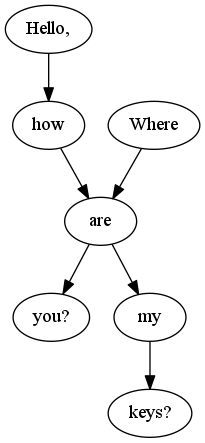
\includegraphics[width=0.2\linewidth]{lab10/example}
  \caption{A graphical representation of the Markov possibilities for ``Hello, how are you?'' and ``Where are my keys?''}
  \label{mark_ex}
\end{figure}

In this graph, each arrow represents a choice we can take based on the last word we added to our sentence, continuing until there are no valid paths to take. Looking at the graph, it's pretty easy to see there are four possible outputs if we start our chain with either ``Hello,'' or ``Where'':

\begin{itemize}
\item Hello, how are you?
\item Hello, how are my keys?
\item Where are you?
\item Where are my keys?
\end{itemize}

For a more complex example, let's use the input phrase ``There is a fifth dimension, beyond that which is known to man. It is a dimension as vast as space and as timeless as infinity.''. If we were to convert this sentence into a graph representing the possible choices to make at each step, it would look something like Figure \ref{twilight}.

\begin{figure}[h]
  \centering
  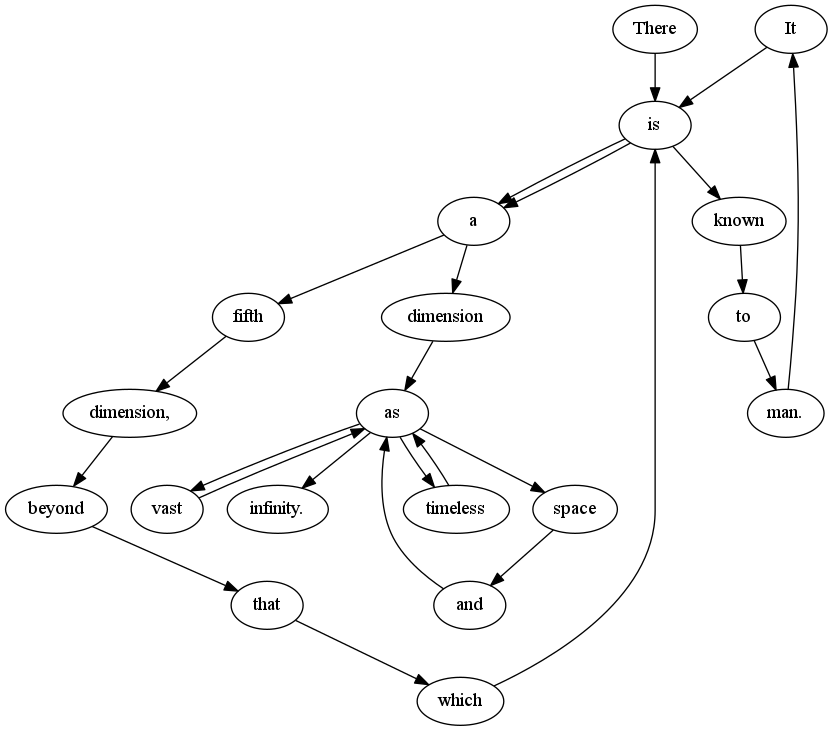
\includegraphics[width=\linewidth]{lab10/twilight_zone}
  \caption{A graphical representation of the Markov possibilities for \emph{The Twilight Zone}'s introduction.}
  \label{twilight}
\end{figure}

In this graph, if we start with ``There'', our only option for a next word is ``is''. ``is'' is followed by ``a'' twice and ``known'' once, so it has two arrows to ``a'' and one to ``known''. This means that, when we randomly choose a next step, we should have a $\frac{2}{3}$ chance to choose ``a'' and a $\frac{1}{3}$ chance to choose ``known''. If we (randomly) choose to continue to ``a'', we have the choice of either ``fifth'' or ``dimension'' to continue our sentence with. A few possible new sentences we could generate from this input are:
\begin{itemize}
\item There is a dimension as infinity.
\item There is a fifth dimension, beyond that which is a fifth dimension, beyond that which is a dimension as vast as space and as infinity.
\item There is known to man. It is known to man. It is a dimension as space and as infinity.
\end{itemize}

As you can see, Markov chains have a tendency to make sentences which almost make sense. This is because every individual pairing of two words will make sense, but the combinations of the pairings might not. For example, ``as vast'' and ``vast as'' can both make sense given the right context, but ``vast as vast as vast as vast'' is nonsense. We can help alleviate this problem by taking into account the last 2 (or 3, or 4...) words when choosing the next word instead of just the last one, but this requires a far larger input or it will result in the output being the same as the input.


\section{Amnesty}
\label{sec:amnesty}
In honor of getting through 10 labs, we are allowing you to resubmit one previous lab for a new grade. If you have a previous lab that you would like to improve your grade on, you may rewrite that lab and upload a new version to be graded. This new grade, if better than your original (hopefully we can assume that will be the case) will replace your original grade.

Upload your redone assignment to the ``Amnesty'' assignment on Canvas.
Make sure it is clear from your filename which lab you are redoing.

\pagebreak

\section{Exercises}
\label{sec:ex}

\begin{warningbox}{Boilerplate}
  Remember that this lab \emph{must} use the
  boilerplate syntax introduced in Lab~5.
\end{warningbox}

\begin{description}
\item[markov.py] Write a program that takes in a filename, reads each line of the file, converts the lines into a format convenient for making Markov chains, and then prints out a new sentence randomly generated from the data, based on the Markov algorithm. When loading the file, treat the lines as separate statements. That is, if ``Hello, how are you?'' and ``Where are my keys?'' are lines in a file, then ``you?'' should not be followed by ``Where'' when generating a chain. However, ``are'' should be allowed to be followed by either ``you?'' or ``my'', as seen in Figure \ref{mark_ex}.

  When creating a new chain, the first element should always be a randomly selected first word of a line in the file. The chain should end when either:
  \begin{itemize}
  \item There are no valid choices to continue the sentence with.
  \item The sentence has reached a length of 100 words.
  \end{itemize}

  You may use any file you wish for test input, though \lstinline{reviews.txt} is provided for you. This is a collection of 12500 reviews from IMDB and is a subset of the data provided at \url{http://ai.stanford.edu/~amaas/data/sentiment/index.html}. When parsing the input file, you should skip any blank lines.
  
\end{description}


\pagebreak
\section{Submitting}

Files to submit:
\begin{itemize}
\item markov.py (Section~\ref{sec:ex})
\item Amnesty Lab (Section~\ref{sec:amnesty})
\end{itemize}

You may submit your code as either a tarball (instructions below) or as a .zip
file. Either one should contain all files used in the exercises for this lab.
The submitted file should be named either
\texttt{cse107\_firstname\_lastname\_lab10.zip} or
\texttt{cse107\_firstname\_lastname\_lab10.tar.gz} depending on which method you
used.

For Windows, use a tool you like to create a \texttt{.zip} file. The TCC
computers should have \texttt{7z} installed. For Linux, look at lab 1 for
instructions on how to create a tarball or use the ``Archive Manager'' graphical
tool.

\begin{center}
  \textbf{Upload your tarball or .zip file to Canvas.}
\end{center}

\end{document}
